\documentclass[oneside,10pt,a4paper]{report}
\usepackage[a4paper, left=3cm, right=3cm, top=3cm, bottom=3cm, headsep=10mm, footskip=12mm]{geometry}
\usepackage[T1]{fontenc}
\usepackage[ngerman, english]{babel}    % mehrsprachiger Textsatz
% babel: letzte Sprache in Optionen zeigt die Sprache des Dokumentes
% und kann durch den Befehl \selectlanguage{} geaendert werden
% Passen Sie die Optionen des babel-Paketes nach Bedarf an!
\usepackage{float}
\usepackage{graphicx}
\usepackage{url}
\usepackage{pdflscape}
\usepackage{mathtools}
\usepackage{amssymb, amsmath, amstext}
\usepackage{amsthm}
\usepackage{xcolor}
\usepackage{nameref}
\usepackage{siunitx}
\usepackage{makecell}
\usepackage{hyperref}
\usepackage{enumitem}
\usepackage[superscript,biblabel]{cite}
\usepackage{caption}
\usepackage{subcaption}
\usepackage{tabularx} 			% Tabellen erzeugen
\usepackage{multirow}			 % Zeilen in Tabellenbearbeitung
\usepackage{multicol} 			% Spalten in Tabellenbearbeitung 
\usepackage{lmodern}                        % Ersatz fuer Computer Modern-Schriften 
\usepackage{amsmath}                                           % zum besseren Aussehen am Bildschirm
\usepackage{booktabs} % für schönere Tabellen
\usepackage{sidecap}
\usepackage{rotating} % für die Landscape-Umgebung
\usepackage{afterpage}
\definecolor{Bluetitle}{HTML}{1F3864}
\definecolor{softbluetitle}{HTML}{274D7E}
\definecolor{Greyish}{HTML}{5A5A5A}
%\renewcommand{\refname}{Reference}
\usepackage{array,multirow}
\newcommand{\specialcell}[2][c]{%
	\begin{tabular}[#1]{@{}c@{}}#2\end{tabular}}
\usepackage{titlesec}

\titleformat{\chapter}[display]
{\normalfont\bfseries}{}{0pt}{\Huge}

\usepackage{lipsum} 


\begin{document}
	
	\begin{titlepage}
		\begin{center}
			\begin{figure}[h!tbp]
				
\includegraphics[width=\linewidth]{HUlogo.PNG}
			\end{figure}
			\vspace*{2 cm}
			
			\textcolor{Bluetitle}{\textbf{\huge Parasitologie - Praktikum}}\par
			
			\vspace*{2cm}
			\textcolor{Greyish}{\textbf{Versuchsdurchführende}}\par
			\textcolor{Greyish}{Huyen Anh Nguyen (572309)}\par

			\vspace*{0.5cm}
			\textcolor{Greyish}{\textbf{Versuchsort}}\par
			\textcolor{Greyish}{Haus 14, Kursraum}\par
			\textcolor{Greyish}{Gruppe 4}\par

			
			\vspace*{2 cm}
			\textcolor{Greyish}{\textbf{Versuchsleiter}}\par
			\textcolor{Greyish}{Prof. Dr. Kai Matuschewski}\par
			\textcolor{Greyish}{\textbf{Versuchsbetreuer}}\par
			\textcolor{Greyish}{Dr. Alexander Maier (ANU)}\par
			\textcolor{Greyish}{Linnea Polito}\par
			\textcolor{Greyish}{Grit Meusel}\par
			\textcolor{Greyish}{Dr. Richard Lucius}\par
			\textcolor{Greyish}{Peer Martin}\par
			\textcolor{Greyish}{Manuel Rauch}\par
			\textcolor{Greyish}{Dr. Katja Müller}\par
			
			
			\textcolor{Greyish}{Abgabe 15. August 2024}\par
			
			
			
		\end{center}
	\end{titlepage}

	
	\tableofcontents
	\chapter{Note from the Author}
	Das Protokoll ist eine Collection von Einzelprotokolle der Versuchen, die in den Parasitologiepraktikum durchgeführt wurde.\\
	Es wurden Methoden gezeigt, wie eine Spezies identifiziert, untersucht und dessen Verhalten analysiert werden kann.\\
	Aufgrund dieser Diversitäten an Versuchen, wird das Protokoll in drei Großkapiteln unterteilt.
	
	
	\chapter{Hirudinea}	
	Hirudinea sind Egel die zu der Klasse Clitellata (Gürtelwürmer, wo auch die Regenwürmer dazuzählen) gehören. Die Arten die zu den Clitellata gehören, besitzen sogenanntes Clitellum, welches das Befruchtungsort für Eizelle und Spermazellen sind. Damit gehören die Tiere in der Klasse Clitella zu den Hermaphroditen.
	Unter den Hirudinea gibt es räuberische Arten (Haemopis sanguisuga) und parasitische Arten (Hirudo verbana), die aquatisch, amphibisch oder auch terrestrisch leben können.
	Morphologisch besitzen die Hirudineas einen Saugnapf am vorderen und einem am hinteren Körperende, wobei der der hintere Saugnapf fürs Anheften gedacht ist und somit größer ist.
	
	\section{Genetische Bestimmung mittels Polymerase-Chain-Reaction}
	\subsection{Einleitung}
	Für die Artenbestimmung des unbekannten Egelgewebeprobe, wird ein genetische Sequence untersucht, das in den Vertebraten konserviert ist. Die Cytocrome C Oxidase subunit 1 (abgekürzt: COI) ist ein konserviertes mitochondrialer
	Gen, das fast alle Tiere besitzen. Die Gen-Sequence weicht von Art zu Art ab und ist daswegen geeignet eine pyhlogenetische Analyse eines Species durchzuführen \cite{Folmer}.
	Für eine gDNA (genomischen DNA) Sequenzierung wird eine bestimmte Menge benötigt, die mittels Polymerase-Chain-Reaction (abgekürzt: PCR) erreicht werden kann.
	Die Polymerase Kettenreaktion (Polymerase Chain-Reaction, abgekürzt: PCR) ist eine Methode, DNA-Abschnitte zu vervielfachen (Amplifikation).
	Für die PCR wird ein hitzestabiles DNA-Polymerase I-Enzym (Taq-Polymerase aus dem Thermus aquaticus-Bekterium) benötigt, da die Doppelsträngige DNA zu Einzelsträngige DNA denaturiert werden muss.
	Für die Amplifikation des 658 bp langes Fragmentes des COI-Sequence, wird als Forward-Primer LCO1490 und Reverse Primer HC02198 verwendet.
	Im Anschluss des PCRs werden die PCR-Produkte über einen Agarosegel nach der Größe aufgetrennt, udn die Bande im Bereich 658 bp isoliert und sequenziert.
	\subsection{Methode}
	\textit{14. Juni 2024}\\
	\\
	Für die gDNA-Isolierung wurde das Genomic DNA tissue kit verwendet.\\
	Ein grobes Stück Egelgewebe (grob 20 mg) wurde mit einem Skalpell homogenisiert und mit 400 $\mu$L Lysispuffer und 25 $\mu$L Proteinase K für 30 Minuten bei 56°C unter Schütteln inkubiert. Dann wurden 250 $\mu$L Bindingsolution SBS zugegeben und gemischt und auf einer Zentrifugenröhrchen überführt. Diese wurde für 2 Minuten bei 10000 x g zentrifugiert und das Filtrat verworfen.\\
	Dann wurde 600 $\mu$L Waschpuffer auf die Säule pipettiert und für 1 Minute für 11000 x g zentrifugiert und dieser Schritt wurde mit 300 $\mu$L Waschpuffer wiederholt. Am Ende des wurde auf maximalen Speed für 30 Sekunden die Überreste an Lösungsmittel abzentrifugiert.\\
	Das Zentrifugenröhrchen wurde auf einem 1.5 mL Eppendorf-Röhrchen überführt und auf dem Filter 50 $\mu$L RNase freies Wasser pipettiert und mit geöffneten Deckel bei 11000 x g für 2 Minuten zentrifugiert.
	\\
	\textit{12. Juli 2024}\\
	\\
	Die Konzentration vom gDNA wurde photometrische bestimmt und beträgt 15.2 mg/mL (Wurde von Grit Meusel durchgeführt).
	Es wurden 2 $\mu$L gDNA und als negativ Kontrolle 2 $\mu$L Wasser mit 23 $\mu$L Mastermix (Pipettierschema für den Mastermix siehe Table \ref{tab: Mastermix-Pipettierschema}).
	Als Primer dient die LCO1490 (5’ GGTCAACAAATCATAAAGATATTGG 3') und HC02198 (5’ TAAACTTCAGGGTGACCAAAAAATCA 3’) Sequenzen von Folmer (1994).
	Die Proben werden dann für 34 Cyclen amplifiziert (PCR-Cyclen siehe Table \ref{tab: PCR-Cyclen}).
	\\
	\textit{14. Juni 2024}\\
	\\
	5 $\mu$L amplfizierte PCR-Proben wird mit 1 $\mu$L 6x Gel-Puffer vermischt und auf einem 1$\%$igen Agarosegel aufgetragen. Zusätzlich wird ein DNA Marker mitraufpipettiert für die Größenbestimmung.
	Der Gellauf lief bei 100V für 1 Stunde und wurde unter ultravioletes Licht analysiert. Die Sequencebestimmung wird von den Versuchsbetreuer durchgeführt.
	
	\subsection{Ergebnis}
	\begin{figure}[H]
		\centering
		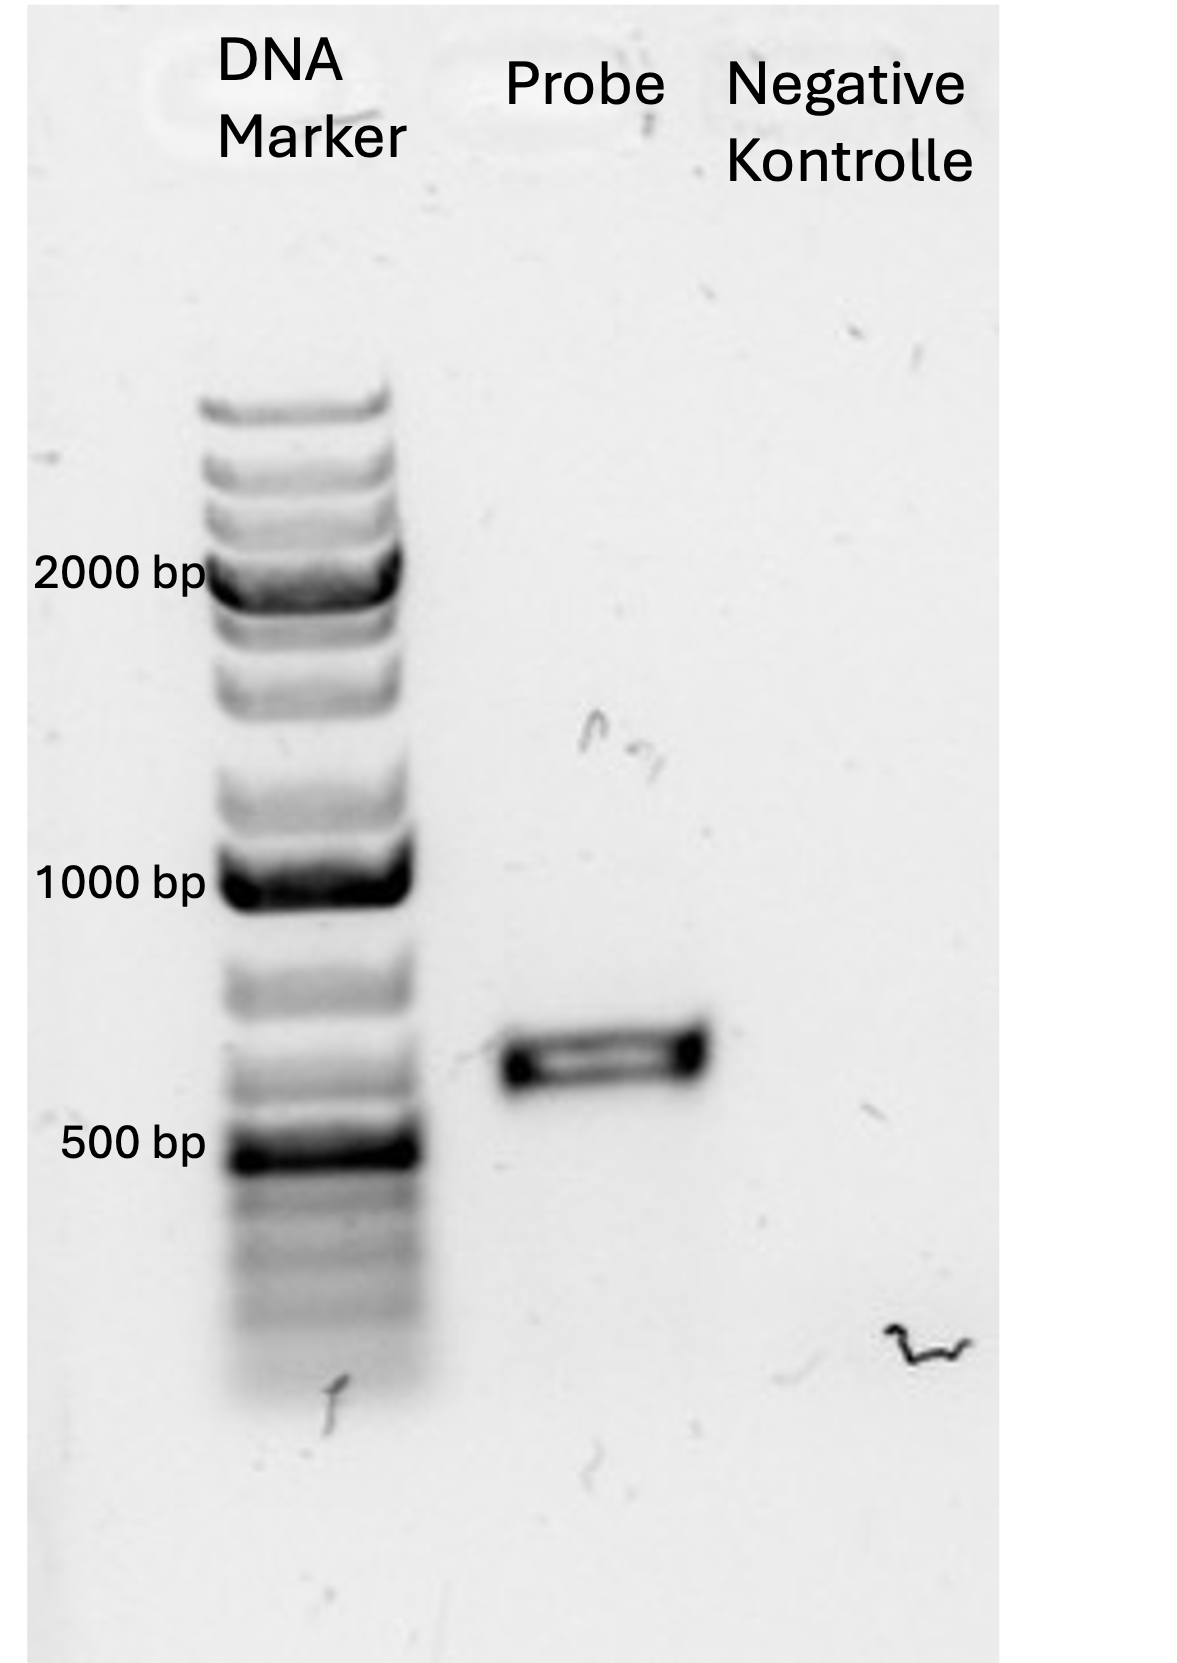
\includegraphics[scale=0.7]{gel.png}
		\caption{Größenauftrennung der gDNA PCR-Probe von der unbekannte Egelgewebestücks und der Negativkontrolle (Wasser) aufgetrennt auf einer 1$\%$-Agarosegel mit einem DNA-Marker als Größenvergleich.}
		\label{fig:Agarosegel}
	\end{figure}
	
	\subsection{Diskusion}
	
	\section{Dichiotomische Bestimmung }
	\subsection{Einleitung}
	\subsection{Methode}
	\subsection{Diskusion}
	
	
	
	\chapter{Trematoden}
	
	
	\chapter{Plasmodium}
	
	\chapter{Anhang}
	\section{PCR}
	\begin{table}[H]
		\centering
		\caption{MasterMix Pipettierschema für 3 PCR-Raktionen. Der MasterMix ist 3-Fach konzentriert}
		\label{tab: Mastermix-Pipettierschema}
		\begin{tabular}{cc}
			\toprule
			& Volumen in $\mu$L\\
			\midrule
			10x Reaktionspuffer & 7.5 \\
			Oligo for & 1.5\\
			Oligo rev & 1.5\\
			dNTP Mix & 1.5\\
			Taq Polymerase & 0.3\\
			H$_2$O & 57\\
			\bottomrule
		\end{tabular}
	\end{table}
	
	
	\begin{table}[H]
		\centering
		\caption{PCR-Cyclus Einstellungsprogramm. 34 Cyclen wurde durchgeführt.}
		\label{tab: PCR-Cyclen}
		\begin{tabular}{cc}
			\toprule
			94°C & 3 Minute\\
			94°C & 45 Sekunde\\
			48°C & 45 Sekunde\\
			72°C & 1 Minute\\
			72°C & 5 Minute\\
			4°C & unendlich\\
			\bottomrule
		\end{tabular}
	\end{table}
	
	
		\addcontentsline{toc}{section}{Bibliography}
	\bibliographystyle{plainurl}
	\nocite{*}
	\bibliography{Literatur}
	\newpage
\end{document}